\documentclass[tikz,border=10pt]{standalone}
\usepackage{amsmath}
\usepackage{amssymb}
\usetikzlibrary{shapes,arrows,positioning,fit,matrix,decorations.pathreplacing,backgrounds}

\begin{document}
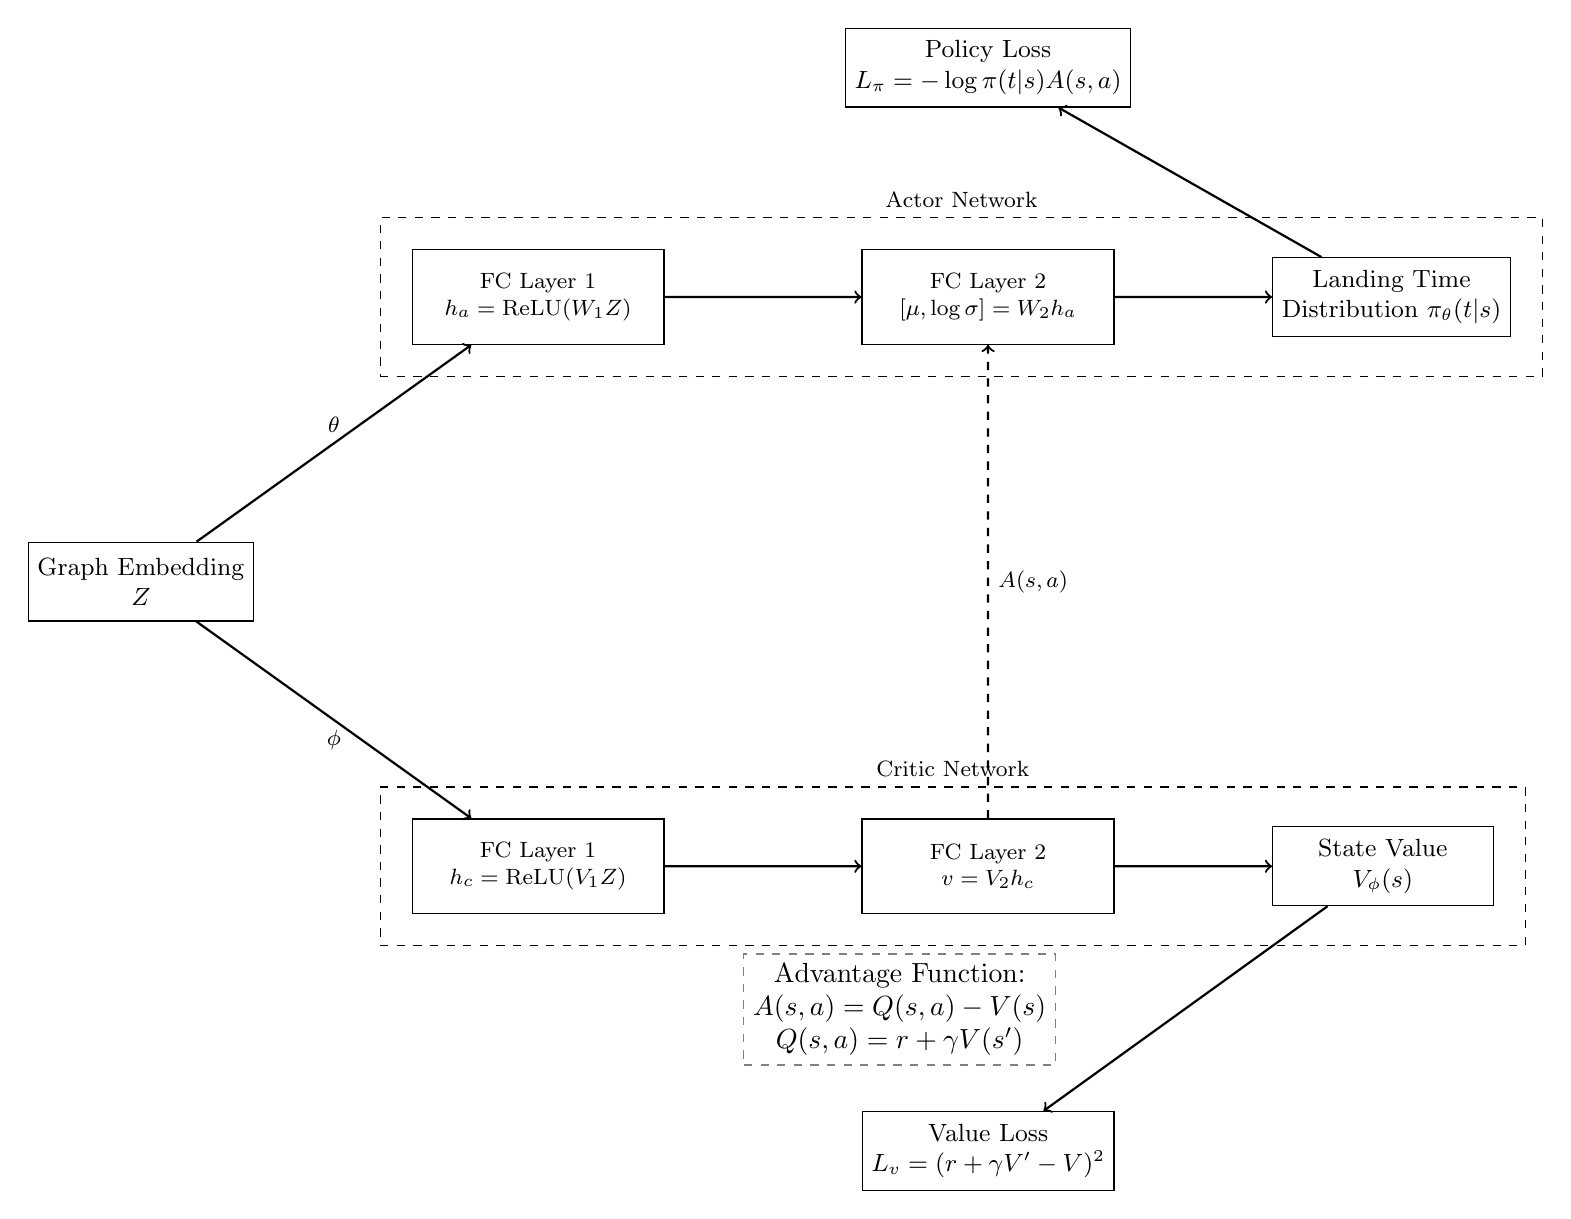
\begin{tikzpicture}[
    scale=0.8,
    node distance=2cm,
    box/.style={
        rectangle,
        draw,
        minimum width=2.8cm,
        minimum height=1cm,
        font=\small,
        align=center
    },
    net/.style={
        rectangle,
        draw,
        minimum width=3.2cm,
        minimum height=1.2cm,
        font=\footnotesize,
        align=center  % Crucial fix for line breaks
    },
    arrow/.style={->,thick}
]

% Input
\node[box] (input) {Graph Embedding\\$Z$};

% Actor Network
\node[net, above right=2.5cm and 2cm of input] (actor1) {
    FC Layer 1\\
    $h_a = \text{ReLU}(W_1Z)$
};
\node[net, right=2.5cm of actor1] (actor2) {
    FC Layer 2\\
    $[\mu,\log\sigma] = W_2h_a$
};
\node[box, right=2cm of actor2] (policy) {
    Landing Time\\
    Distribution $\pi_\theta(t|s)$
};

% Critic Network
\node[net, below right=2.5cm and 2cm of input] (critic1) {
    FC Layer 1\\
    $h_c = \text{ReLU}(V_1Z)$
};

\node[net, right=2.5cm of critic1] (critic2) {  % Fixed node name
    FC Layer 2\\
    $v = V_2h_c$
};
\node[box, right=2cm of critic2] (value) {
    State Value\\
    $V_\phi(s)$
};


% Losses
\node[box, below=2.5cm of critic2] (vloss) {
    Value Loss\\
    $L_v = (r + \gamma V' - V)^2$
};
\node[box, above=1.8cm of actor2] (ploss) {
    Policy Loss\\
    $L_\pi = -\log\pi(t|s)A(s,a)$
};

% Advantage Calculation
\node[draw=black!50, dashed, align=center, below right=0.5cm and 1cm of critic1] (advantage) {
    Advantage Function:\\
    $A(s,a) = Q(s,a) - V(s)$\\
    $Q(s,a) = r + \gamma V(s')$
};

% Connections
\draw[arrow] (input) -- node[above,font=\footnotesize] {$\theta$} (actor1);
\draw[arrow] (actor1) -- (actor2);
\draw[arrow] (actor2) -- (policy);
\draw[arrow] (input) -- node[below,font=\footnotesize] {$\phi$} (critic1);
\draw[arrow] (critic1) -- (critic2);
\draw[arrow] (critic2) -- (value);
\draw[arrow] (policy) -- (ploss);
\draw[arrow] (value) -- (vloss);

% Advantage connection
\draw[arrow, dashed] (critic2) -- node[right,font=\footnotesize] {$A(s,a)$} (actor2);

% Background boxes
\begin{pgfonlayer}{background}
    \node[rectangle,draw,dashed,fit=(actor1)(actor2)(policy),
          inner sep=0.4cm,
          label={[above,font=\footnotesize]Actor Network}] {};
    \node[rectangle,draw,dashed,fit=(critic1)(critic2)(value),
          inner sep=0.4cm,
          label={[above,font=\footnotesize]Critic Network}] {};
\end{pgfonlayer}

\end{tikzpicture}
\end{document}
